%\vspace{-2ex}
\section{Overview}
\label{sec:Overview}
%\vspace{-.1in}
%\begin{figure}[t]
%\vspace{-0.5in}
%\centering
%\psfig{figure=figures/plots/runtimeFinal.eps,width=5.5in} }
%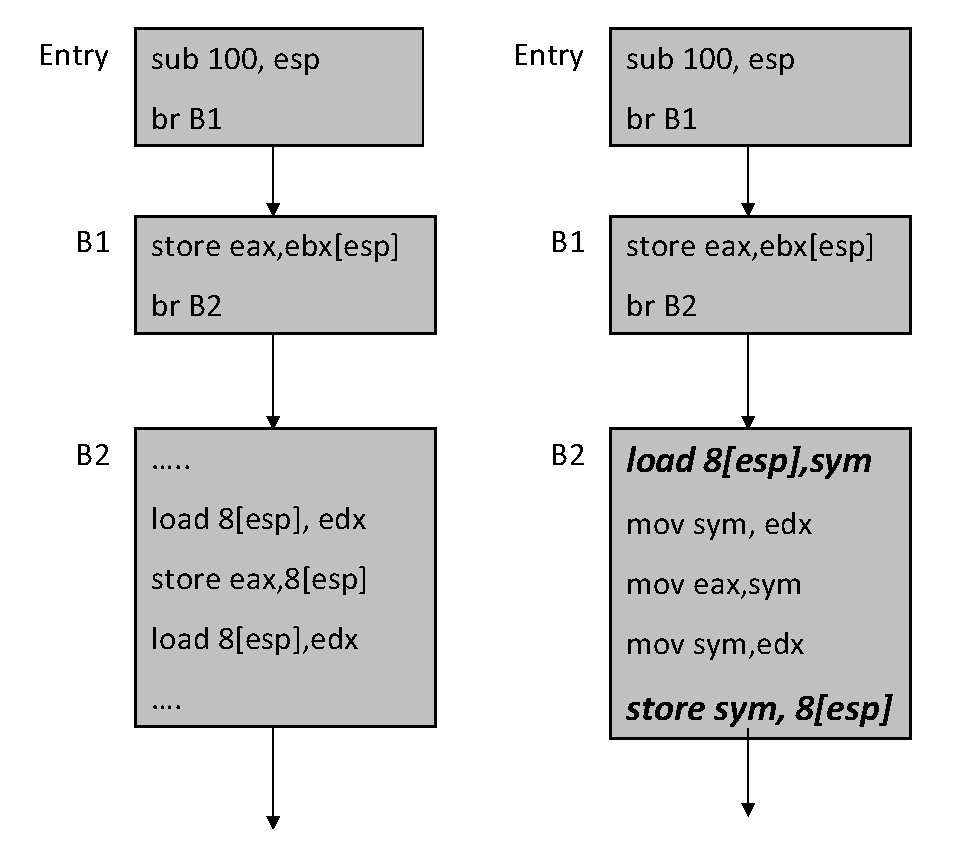
\includegraphics [width=0.5\linewidth] {figures/EPS/cfgex.eps} 
%\tiny{
%\caption { \textit{Stack layout in a binary}}
%}
%\label{fig:stack-layout}
%\end{figure}

\begin{figure}[t]
{
%\begin{minipage}{.5\linewidth}
{
\centering
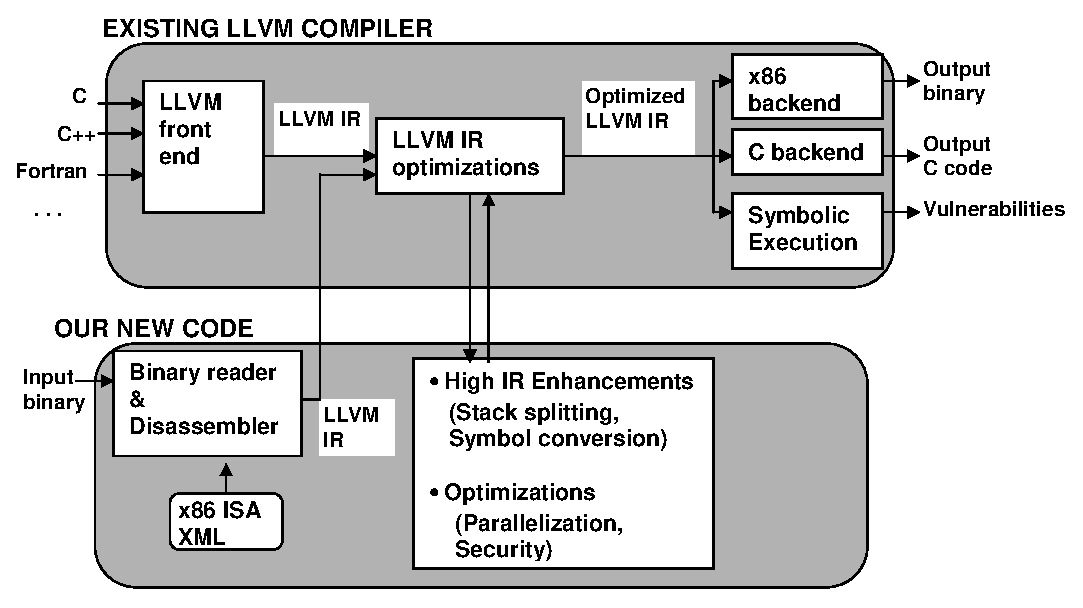
\includegraphics[width=0.7\linewidth]{figures/EPS/flow1.eps}
\caption{\scriptsize{System Flow}}
\label{fig:systemflow}
\vspace{-0.2in}
}
%\end{minipage}
\hfill
%\begin{minipage}{0.3\linewidth}
%{
%\centering
%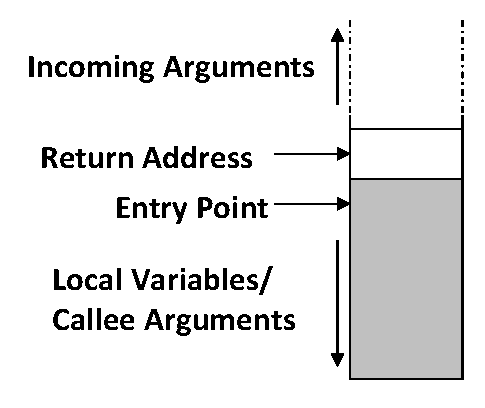
\includegraphics[width=\linewidth]{figures/EPS/stackLayout1.eps} 
%\caption{A typical stack layout}
%\label{fig:stacklayout}
%}
%\end{minipage}
\vspace{-0.2in}
}
\end{figure}

Fig~\ref{fig:systemflow} presents an overview of the \emph{SecondWrite} system. SecondWrite produces LLVM IR using our custom binary reader modules. SecondWrite can be used as a binary rewriter by using the x86 back-end, or as a binary $\rightarrow$ C converter by using LLVM's existing C back-end.
%The frontend module in \emph{SecondWrite} system, consisting of a disassembler and a custom reader module, processes the individual instructions in input executable and generates an initial LLVM IR. This initial representation is devoid of the desired IR features like abstract stack frame and symbols. This initial IR is analyzed to obtain an improved IR which has all the information and features mentioned previously. The standard suite of LLVM optimizations and various new optimization passes can be applied on the above IR to get an optimized IR. The optimized IR is finally passed to the existing LLVM code generator to obtain the rewritten binary. The C backend present in LLVM compiler can be used to obtain C code for better analysis of executables.
%\footnote{Indirect calls and branches occurring in the original binary are handled by translating their target addresses in relocation tables when present in the binary, or through a custom binary rewriting technique we are developing when such tables are absent. However, the choice of technique is orthogonal to the techniques presented in this paper and does not affect our analysis}. 



